%! Author = gra
%! Date = 23.03.24

% Preamble
\begin{flushleft}
    \subsubsection{Benchmarking - Vorgehen}
    \paragraph{YugabyteDB}
    Zuerst muss die Datenbank erstellt und die Tablespaces erzeugt werden, die genauen Schritte sind im \hyperref[subsubsec:yugabytedb_benchmarking_sql]{Anhang - YugabyteDB Benchmark SQL} zu finden.\\    Anschliessend
    Anschliessend muss pro Lauf erst initialisiert werden, dann kann mit dem eigentlichen Benchmarking gestartet werden.\\
    Alle Benchmarking-Commands sind im \hyperref[subsec:yugabytedb_benchmarking_commands]{Anhang - YugabyteDB Benchmarking Commands} zu finden.
    \paragraph{Patroni}
    Als die 250GiB DB getestet wurde, zeigte sich, dass die Parameter nicht darauf optimiert waren.

    \paragraph{StackGres - Citus}
    Beim Benchmarking zeigten sich die Grenzen des Citus Shardings.\\
    Bereits beim Lesen der Anleitung fiel auf, dass für das Sharding der Tabellen \texttt{pgbench\_accounts} und \texttt{pgbench\_history} jeweils neu initialisiert wurde\cite{6CJFR7RM}.\\
    Das hat einen besonderen Grund.\\
    Wenn die Tabellen mittels des SELECT-Statements \texttt{create\_distributed\_table} die Tabellen einem Sharding unterzogen werden sollen, kommt es zu einer Fehlermeldung.\\
    Die Shards würden mit folgenden SQL-Statements erzeugt:
\lstset{style=gra_codestyle}
\begin{lstlisting}[language=sql, caption=Citus - Benchmarking - Distributed Table Sharding,captionpos=b,label={lst:benchmarking_distributed_table_sharding},breaklines=true]
SELECT create_distributed_table('pgbench_branches', 'bid');
SELECT create_distributed_table('pgbench_tellers', 'tid');
SELECT create_distributed_table('pgbench_accounts', 'aid');
SELECT create_distributed_table('pgbench_history', 'aid');
\end{lstlisting}
    Ursache ist, dass eine Distributed Table offenbar keine Foreign Key Constraints erlaubt.\\
    \texttt{pgbench} erzeugt aber gleich mehrere davon:\\
    \begin{figure}[H]
        \centering
        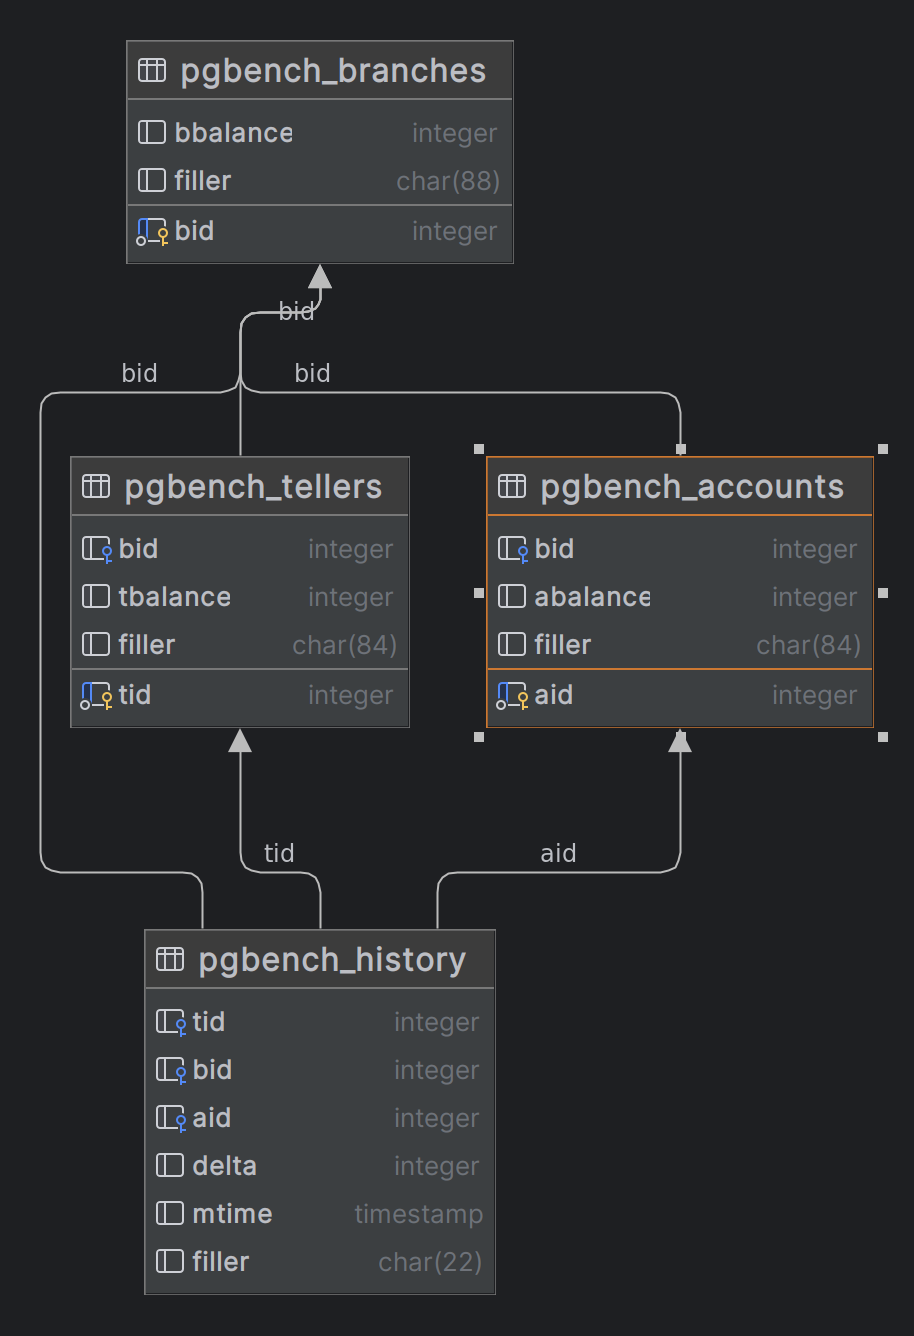
\includegraphics[width=0.5\linewidth]{source/implementation/evaluation/benchmarking/stackgres_citus/pgbench_accounts}
        \caption{Benchmarking - ERD pgbench}
        \label{fig:pgbench_accounts}
    \end{figure}
    Ein Schema-Based Sharding ist nicht möglich, da \texttt{pgbench} nur die DB als Parameter übernimmt.\\
    Die Tabellen werden zudem immer dropped bevor sie neu erzeugt und gefüllt werden, das Sharding kann daher nur im Nachgang gemacht werden.\\
\end{flushleft}
\begin{flushleft}
    Die Lösung für das Benchmarking bestand also darin, sogenannte Reference Tables zu erstellen:
\lstset{style=gra_codestyle}
\begin{lstlisting}[language=sql, caption=Citus - Benchmarking - Reference Table Sharding,captionpos=b,label={lst:benchmarking_reference_table_sharding},breaklines=true]
SELECT create_reference_table('pgbench_branches');
SELECT create_reference_table('pgbench_tellers');
SELECT create_reference_table('pgbench_accounts');
SELECT create_reference_table('pgbench_history');
\end{lstlisting}
    Referenzierte Tabellen werden auf alle Shards repliziert und erfüllen somit die Anforderung an das Sharding.\\
    Diese Art des Sharding wäre allerdings nur für kleinere Tabellen, Multi-Tenant Sharding (wenn Tabellen bei allen Tenants verfügbar sein sollen),\\
    Tabellen die mit verschiedenen Distributed Tables gejoint werden oder wenn eben, wie in unserem Fall, Foreign-Key Constraints im Spiel sind\cite{KPPLMKD4}.
\end{flushleft}
\begin{flushleft}
    Aber auch in diesem Fall muss das Sharding im Nachgang des \texttt{pgbench}-Inits gemacht werden.\\
    Bei den kleinen Tabellen geht das relativ flot, doch gerade bei der Tabelle \texttt{pgbench\_accounts} dauert es sehr lange.\\
    Lang genug, dass eine eigene betrachtung beim Benchmarking angezeigt wurde.\\
    Leider zeigte sich auch bei den mixed-Benchmarks, anders als bei den dql-Benchmarks, dass diese Art des Sharding nicht sehr performant ist.
\end{flushleft}
\begin{flushleft}
    Wie bei Patroni und YugabyteDB auch, musste für den letzten Benchmark die StorageClass auf die neue Disk verlegt werden.\\
    Aber anders als bei YugabyteDB reichten 250GiB nicht mehr, wie bei Patroni lag die Ursache beim Generieren der Primary- und Foreign-Keys.
\end{flushleft}
\begin{flushleft}
    Es zeigte sich aber auch rasch, dass der Coordinator die gleiche Grösse annahm, wie die Shard-Pods.\\
    Das führte dazu, dass beim letzten Benchmark nur noch 2 Shard-Instanzen deployt werden konnten,\\
    da sonst bei jeder Disk nochmals mindestens 350GiB hinzugefügt hätte werden müssen (da sich der Coordinator den Node mit einem Shard geteilt hätte und der Coordinator auf jedem Node erscheinen könnte).\\
    Es hätten also für die Evaluation 3 x 700GiB (plus noch 3 x 50GiB für den Rest), also 3 x 750GiB, allokiert werden müssen.\\
    Auf diesen Mehraufwand wurde verzichtet um das \Gls{SAN} und somit das Daily Business nicht zu stark zu belasten.
\end{flushleft}
\begin{flushleft}
    Alle Benchmarking-Commands und SQLs zur ermittlung der grösse sind im \hyperref[subsec:stackgres_citus_benchmarking_commands]{Anhang - StackGres - Citus Benchmarking Commands} zu finden.
    \subsubsection{Benchmarks}
    Der vergleich zwischen den verschiedenen Varianten.\\
\end{flushleft}
\begin{flushleft}

\end{flushleft}
\begin{flushleft}
    Bei den Transaktionen pro Sekunden gilt, je höher der Wert, umso besser das Ergebnis.\\
%    Zuerst die Ergebnisse mit den mixed-Transaktionen:
%    \begin{figure}[H]
%        \centering
%        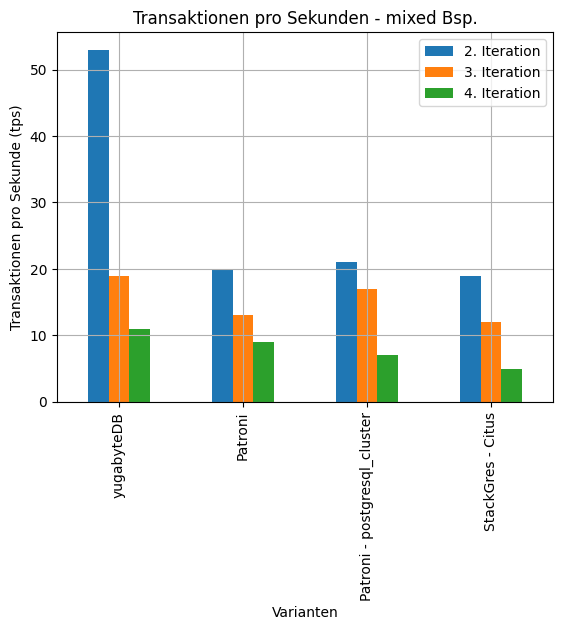
\includegraphics[width=0.5\linewidth]{source/pandas_data_chart_plotter/tps_mixed}
%        \caption{Benchmarks - tps mixed}
%        \label{fig:tps_mixed}
%    \end{figure}
%
%    Folgend die reinen Select-Transaktionen.
%    \begin{figure}[H]
%        \centering
%        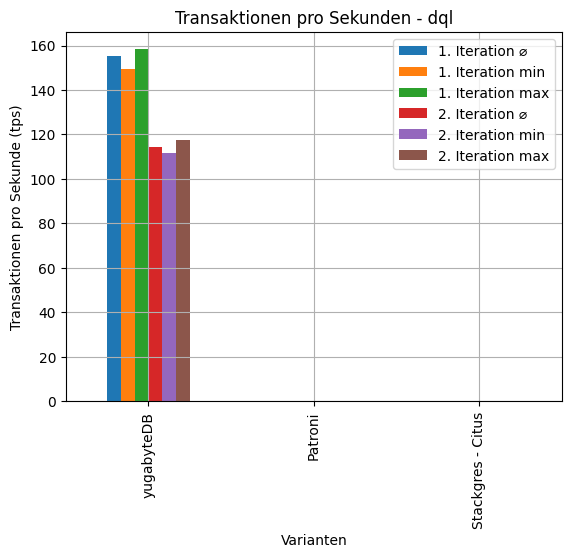
\includegraphics[width=0.5\linewidth]{source/pandas_data_chart_plotter/tps_dql}
%        \caption{Benchmarks - tps dql}
%        \label{fig:tps_dql}
%    \end{figure}

    \begin{figure}[H]
        \centering
        \subfloat{{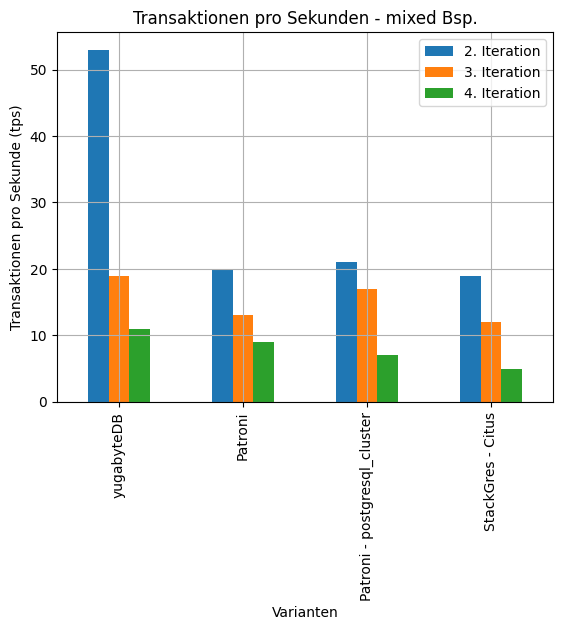
\includegraphics[width=0.47\linewidth]{source/pandas_data_chart_plotter/tps_mixed} }}%
        \qquad
        \subfloat{{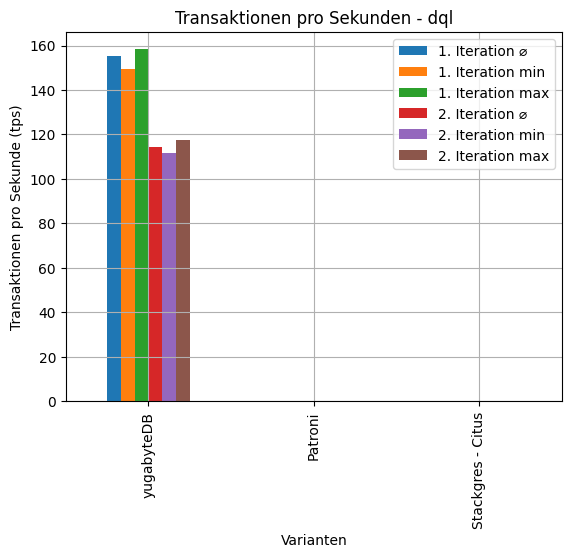
\includegraphics[width=0.47\linewidth]{source/pandas_data_chart_plotter/tps_dql} }}%
        \caption{Benchmarks - tps}
        \label{fig:tps_varianten}
    \end{figure}
    Bei der Latenz ist es genau andersrum, je höher der Wert desto schlechter schnitt die Variante ab.\\
%    Auch hier zuerst wieder die mixed-Transaktionen:
%    \begin{figure}[H]
%        \centering
%        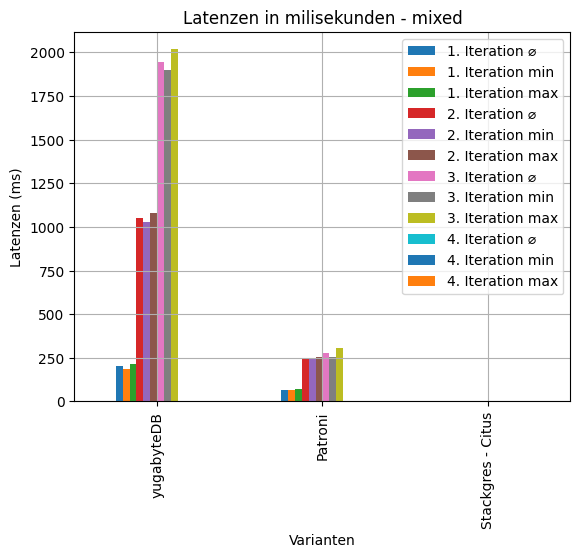
\includegraphics[width=0.5\linewidth]{source/pandas_data_chart_plotter/latency_mixed}
%        \caption{Benchmarks - latency mixed}
%        \label{fig:latency_mixed}
%    \end{figure}
%
%    Folgend die Select-Transaktionen:
%    \begin{figure}[H]
%        \centering
%        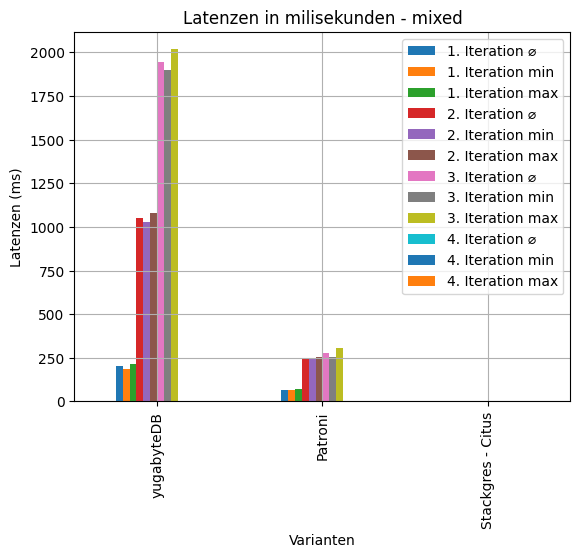
\includegraphics[width=0.5\linewidth]{source/pandas_data_chart_plotter/latency_dql}
%        \caption{Benchmarks - latency dql}
%        \label{fig:latency_dql}
%    \end{figure}

    \begin{figure}[H]
        \centering
        \subfloat{{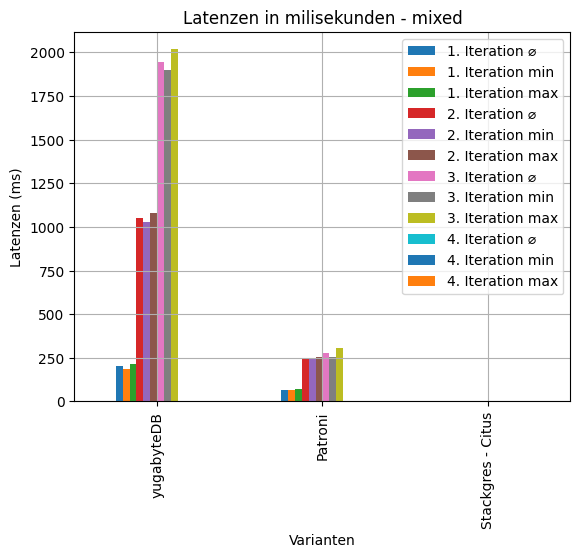
\includegraphics[width=0.47\linewidth]{source/pandas_data_chart_plotter/latency_mixed} }}%
        \qquad
        \subfloat{{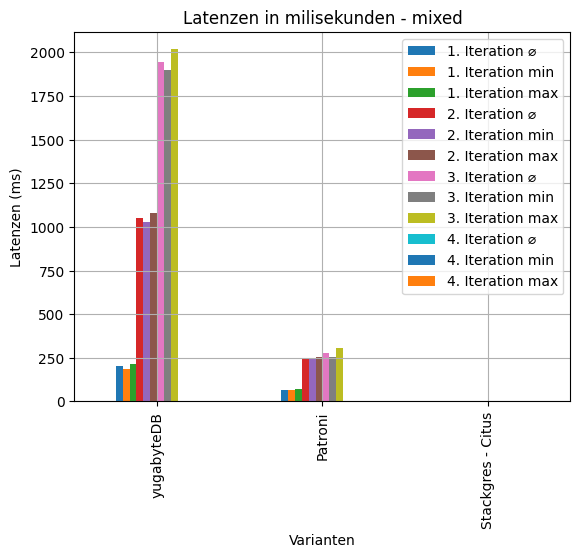
\includegraphics[width=0.47\linewidth]{source/pandas_data_chart_plotter/latency_dql} }}%
        \caption{Benchmarks - latency}
        \label{fig:latency_varianten}
    \end{figure}
\end{flushleft}
\begin{flushleft}
    Die ersten beiden läufe mit Patroni wurde erst nur mit der Asynchronen Standard-Replikation von Patroni vorgenommen.\\
    Später wurden die Benchmarks mit der Synchronen Replikation wiederholt.\\
    Daraus ergab sich die Möglichkeit, beide Methoden direkt zu vergleichen:
    \begin{figure}[H]
        \centering
        \subfloat{{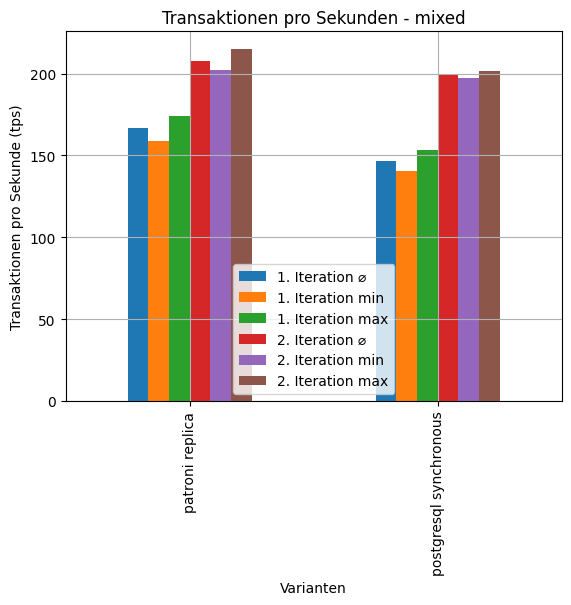
\includegraphics[width=0.47\linewidth]{source/pandas_data_chart_plotter/tps_patroni_replica_mixed} }}%
        \qquad
        \subfloat{{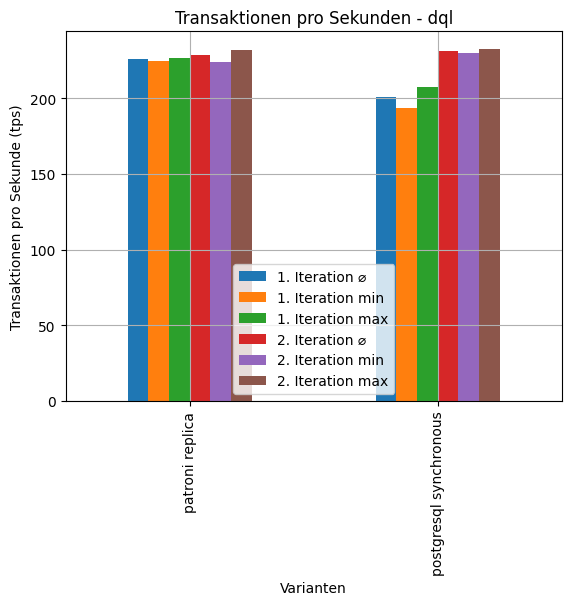
\includegraphics[width=0.47\linewidth]{source/pandas_data_chart_plotter/tps_patroni_replica_dql} }}%
        \caption{Benchmarks - tps Patroni Replica}
        \label{fig:tps_patroni_replica}
    \end{figure}
    \begin{figure}[H]
        \centering
        \subfloat{{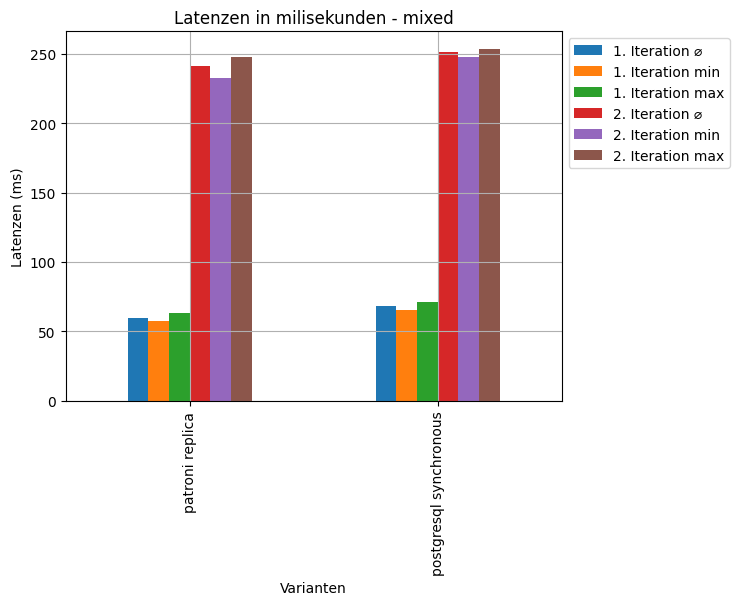
\includegraphics[width=0.47\linewidth]{source/pandas_data_chart_plotter/latency_patroni_replica_mixed} }}%
        \qquad
        \subfloat{{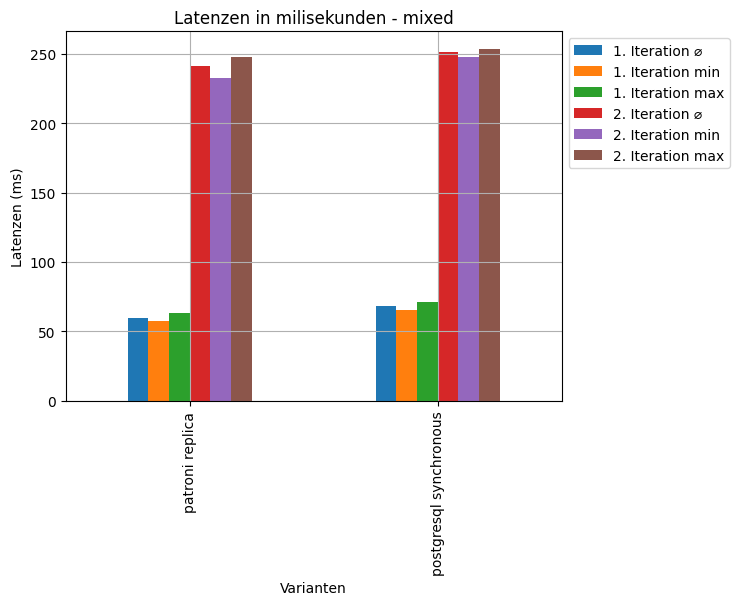
\includegraphics[width=0.47\linewidth]{source/pandas_data_chart_plotter/latency_patroni_replica_dql} }}%
        \caption{Benchmarks - latency Patroni Replica}
        \label{fig:latency_patroni_replica}
    \end{figure}
    Die Asynchrone Replikation ist dabei ein klein wenig schneller als die Synchrone Replikation.
\end{flushleft}
\begin{flushleft}
    Ein weiterer Benchmark sind die Fehler, die bei den DML-Transktionen beim mixed-Benchnmark auftreten können.
    \begin{figure}[H]
        \centering
        \subfloat{{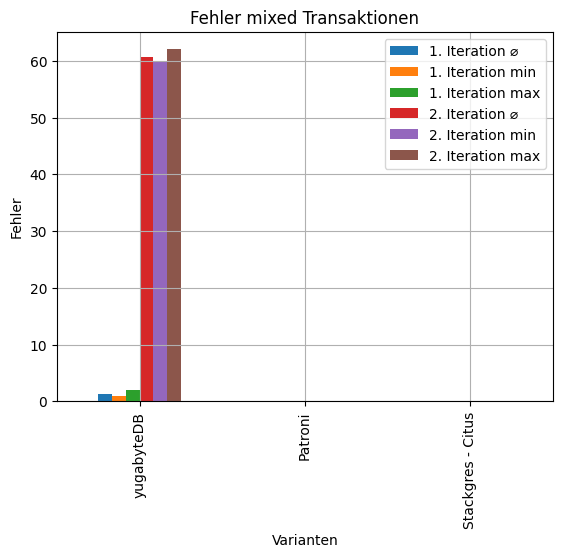
\includegraphics[width=0.47\linewidth]{source/pandas_data_chart_plotter/pgbench_errors_absolute} }}%
        \qquad
        \subfloat{{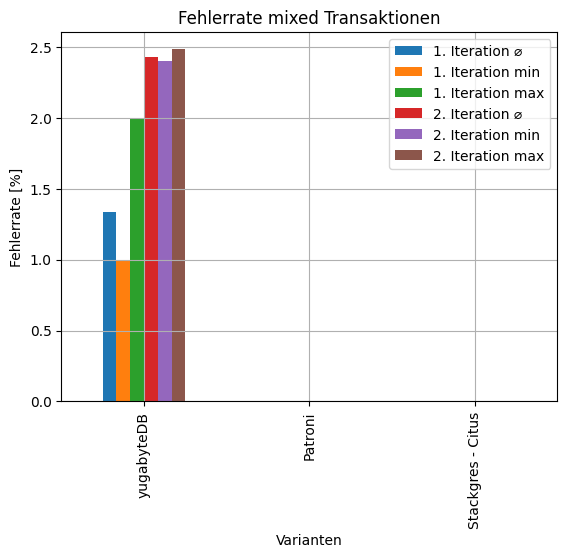
\includegraphics[width=0.47\linewidth]{source/pandas_data_chart_plotter/pgbench_errors_percentage} }}%
        \caption{Benchmarks - Fehler bei mixed-Transaktionen}
        \label{fig:pgbench_errors}
    \end{figure}
\end{flushleft}
\begin{flushleft}
    Ebenfalls ein wichtiger Benchmark ist die Zeit, die benötigt wird, um mittels \texttt{pgbench} initialisiert die Tabellen zu erstellen.
    \begin{figure}[H]
        \centering
        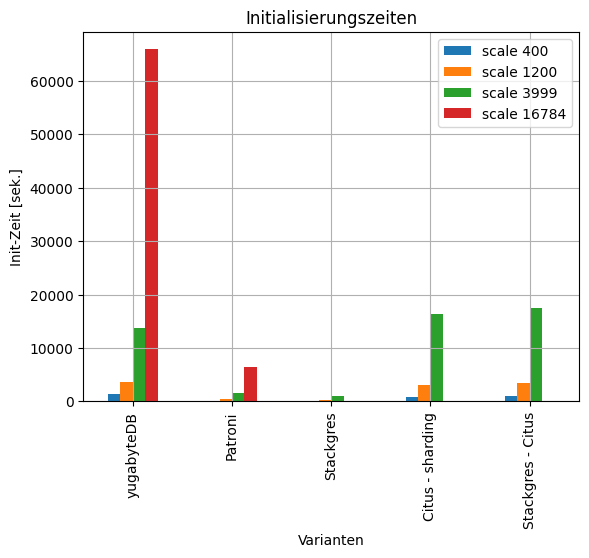
\includegraphics[width=0.5\linewidth]{source/pandas_data_chart_plotter/initializing_time_sec}
        \caption{Benchmarks - Initialisierungszeit - sekunden}
        \label{fig:initializing_time_sec}
    \end{figure}
    \begin{figure}[H]
        \centering
        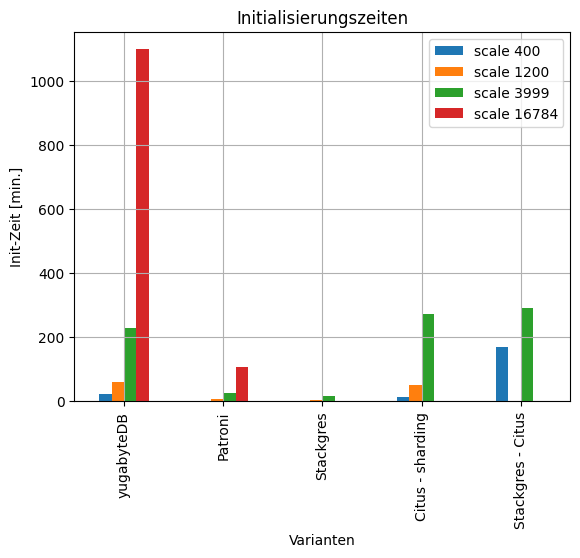
\includegraphics[width=0.5\linewidth]{source/pandas_data_chart_plotter/initializing_time_min}
        \caption{Benchmarks - Initialisierungszeit - minuten}
        \label{fig:initializing_time_min}
    \end{figure}
    \begin{figure}[H]
        \centering
        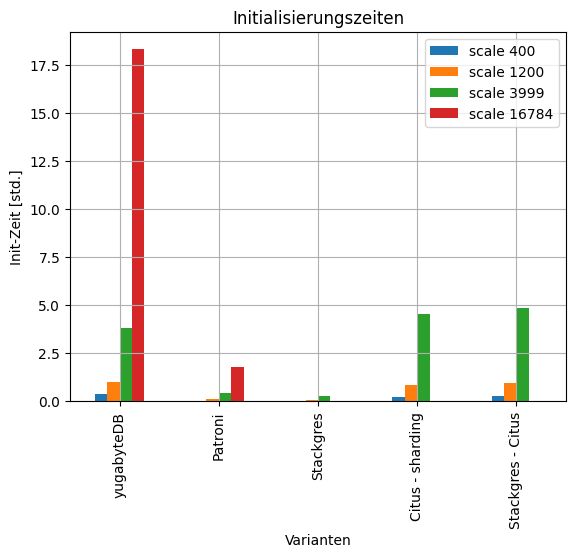
\includegraphics[width=0.5\linewidth]{source/pandas_data_chart_plotter/initializing_time_hour}
        \caption{Benchmarks - Initialisierungszeit - stunden}
        \label{fig:initializing_time_hour}
    \end{figure}
    Dabei fällt auf, mit Patroni werden die Tabellen am schnellsten geladen.\\
    StackGres selber generiert ebenfalls wesentlich schneller als YugabyteDB.\\
    Werden dann aber die Tabellen in Shards aufgeteilt, verändert sich die Initialisierungszeit zuungunsten von StackGres - Citus.


\end{flushleft}
